\documentclass[12pt,a4paper,openright,twoside]{book}
\usepackage[utf8]{inputenc}
\usepackage{disi-thesis}
\usepackage{code-lstlistings}
\usepackage{notes}
\usepackage{shortcuts}
\usepackage{acronym}

\school{\unibo}
\programme{Corso di Laurea Magistrale in Ingegneria e Scienze Informatiche}
\title{Fancy Title}
\author{Alberto Donati}
\date{\today}
\subject{Supervisor's course name}
\supervisor{Prof. Supervisor Here}
\cosupervisor{Dott. CoSupervisor 1}
\morecosupervisor{Dott. CoSupervisor 2}
\session{IV}
\academicyear{2022-2023}

% Definition of acronyms
\acrodef{IoT}{Internet of Thing}
\acrodef{vm}[VM]{Virtual Machine}


\mainlinespacing{1.241} % line spacing in mainmatter, comment to default (1)

\begin{document}

\frontmatter\frontispiece

\begin{abstract}

    Considering that companies have an increasing number of server connected to the network, IT professionals increasingly find themselves with machines on which to perform the same tasks.
    Therefore, systems that could automate tasks on large numbers of machines in parallel have been created and are increasingly being used.
    This thesis aims to compare and evaluate different server automation and orchestration systems, analyzing their features, advantages, and disadvantages.
    It will then go on to provide a summary overview of the reasons why professionals choose one alternative over another.
\end{abstract}

%\begin{dedication} % this is optional
%Optional. Max a few lines.
%\end{dedication}

%\begin{acknowledgements} % this is optional
%Optional. Max 1 page.
%\end{acknowledgements}

%----------------------------------------------------------------------------------------
\tableofcontents   
\listoffigures     % (optional) comment if empty
\lstlistoflistings % (optional) comment if empty
%----------------------------------------------------------------------------------------

\mainmatter

%----------------------------------------------------------------------------------------
\chapter{Introduction}
\label{chap:introduction}
%----------------------------------------------------------------------------------------

This thesis aims to compare and evaluate different server automation and orchestration systems.
It will provide also a summary overview, useful for professionals of IT to compare solutions.

\paragraph{Structure of the Thesis}

\note{At the end, describe the structure of the paper}

\chapter{State of the art}

\section{What are automation systems}
Automation systems are software tools that allow you to manage, monitor, and automate operations on a large number of servers. These systems can include features such as automatic provisioning, configuration management, service orchestration, performance monitoring, and troubleshooting.
An example of these systems is \textbf{Ansible}, which uses an agentless management model to connect to servers and perform automation tasks. Other examples include Puppet, Chef, and SaltStack, which offer similar features but use different approaches for server management.
These automation systems can be particularly useful in environments with a large number of servers, where manual management of each server would be inefficient and prone to errors. Through automation, organizations can improve operational efficiency, reduce errors, and free up IT staff to focus on other works.
Automation systems aims to simplify the execution of repetitive task.

\section{Who uses automation systems}

\section{When it makes sense (or doesn't make sense) to automate operations}

\section{What are the main systems}

\section{OpenSource and Closed Source, when OpenSource becomes Closed for some use cases}

%I suggest referencing stuff as follows: \cref{fig:random-image} or \Cref{fig:random-image}

%\begin{figure}
%    \centering
%    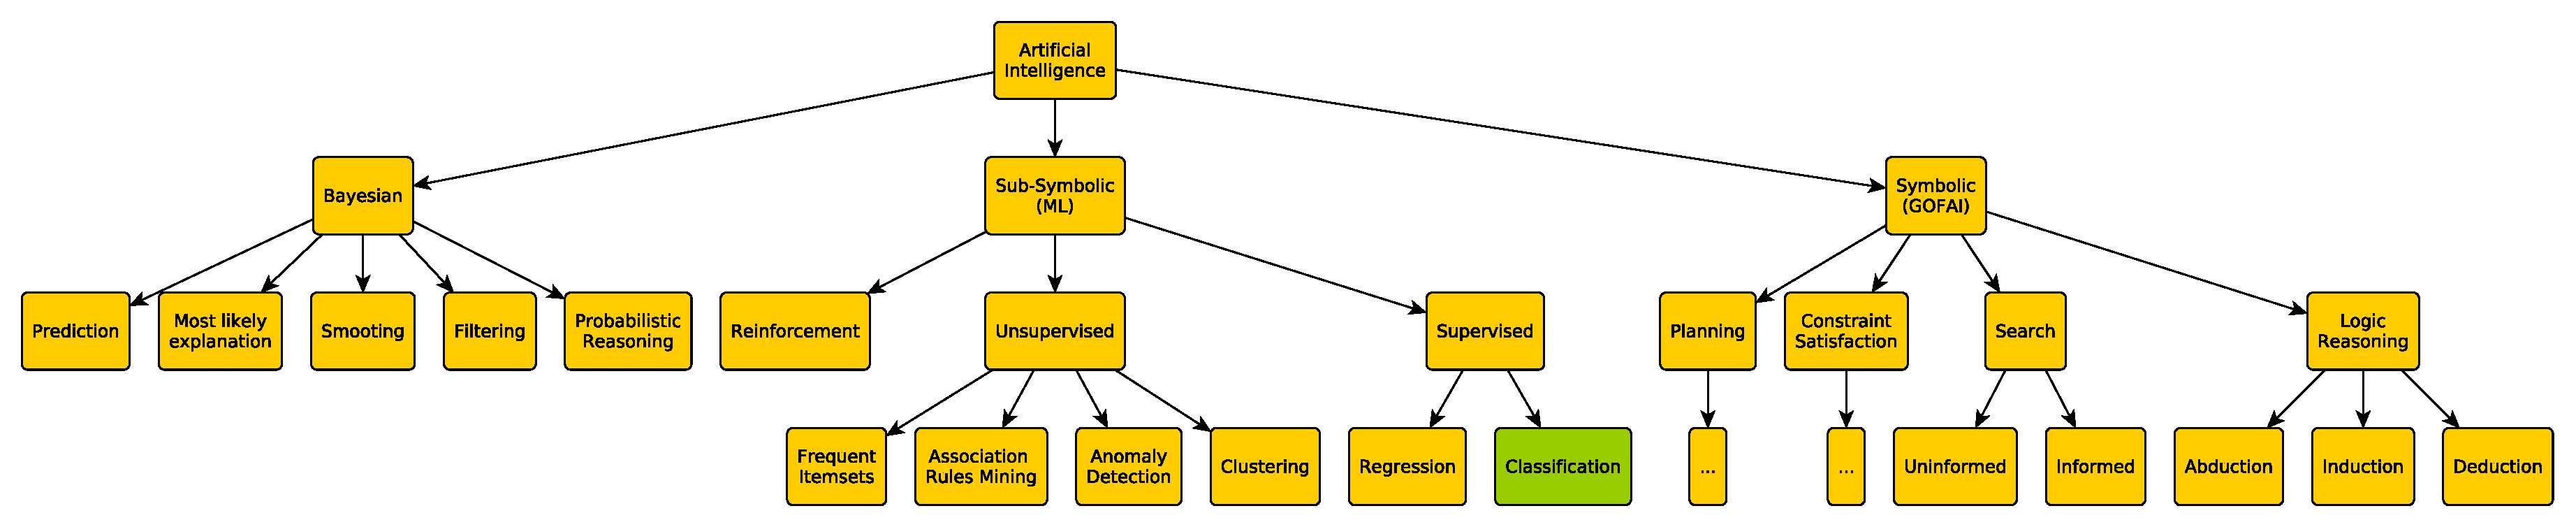
\includegraphics[width=.8\linewidth]{figures/random-image.pdf}
%    \caption{Some random image}
%    \label{fig:random-image}
%\end{figure}

%\begin{document}

\section{Conclusion of the research}
Scrivere la conclusione

\subsection{Comparations}
Esempio comparazione tecnologie

\subsection{Consideration}
Considerazioni finali

\end{document}

%\section{Some cool topic}

\chapter{Contribution}

You may also put some code snippet (which is NOT float by default), eg: \cref{lst:random-code}.

\lstinputlisting[float,language=Java,label={lst:random-code}]{listings/HelloWorld.java}

%\section{Fancy formulas here}

%----------------------------------------------------------------------------------------
% BIBLIOGRAPHY
%----------------------------------------------------------------------------------------

\backmatter

\nocite{*} % comment this to only show the referenced entries from the .bib file

\bibliographystyle{alpha}
\bibliography{bibliography}

\end{document}